\chapter{Power Series}\label{PowerSeries}

\section{Wouldn't It Be Nice If All Functions Were Polynomials?}  Think about say, differentiating and antidifferentiating.  It becomes difficult when rational functions, trigonometric functions, logarithms, and exponentials are involved.  If every function were just polynomial, calculus would be much easier!

\series{Power series} is an attempt to make this dream a reality and turn these non-polynomial functions into polynomials!  There is just one slight hangup; it is mathematically impossible.  For example...

\begin{theorem}{Cosine Cannot Be Written as a Polynomial}
Cosine cannot be written as a polynomial.
\end{theorem}
\vspace{-.1in}
\begin{proof} Let $n$ be a natural number.  By the Fundamental Theorem of Algebra, a degree $n$ polynomial has at most $n$ roots.  However, $\cos(x)$ has infinitely many roots.  Thus, the cosine function cannot be equal to any polynomial, since no polynomial has infinitely many roots.
\end{proof}

Unphased by minor complications like something being impossible, we proceed anyway.  If polynomials can only have as many roots as their degree and cosine needs infinitely many roots, maybe we just need to allow polynomials to have infinite degree!  This is exactly the \powerseries{definition} of a \emph{power series}.  A power series is simply a polynomial whose degree is allowed to be infinite.  Let's say this again but more formally.

\begin{definition}{Power Series}
A \emph{power series} is an expression of the form $$a_0+a_1x+a_2x^2+a_3x^3+a_4x^4+a_5x^5+\cdots $$ for real or complex numbers $a_i$.
\end{definition}

Many other sources refer to the above as a \emph{Maclaurin Series}, or a \emph{Taylor Series Centered at Zero}.  Since it is a sum of powers of $x$, we stick with the simple descriptive name, \taylorseries{\maclaurin{power series}}.

\begin{example}{The Power Series for Cosine, One Coefficient at a Time}
We return to our original goal!  Since we cannot find a finite degree polynomial equal to the cosine function, we instead find an infinite degree polynomial (aka \cosine{power series}) for cosine.  We desire $a_i$ such that

$$\cos(x)=a_0+a_1x+a_2x^2+a_3x^3+a_4x^4+a_5x^5+\cdots. $$
We solve for the coefficients $a_i$ one at a time.
\begin{itemize}
\item {\bf Solving for $a_0$:} We certainly want this formula to be true for $x=0$, so let's plug $x=0$ into both sides and see what happens.

$$\cos(0)=a_0+a_1\cdot 0+a_2\cdot 0^2+a_3\cdot 0^3+a_4\cdot 0^4+a_5\cdot 0^5+\cdots $$
$$1=a_0 $$

Thus, we found our first coefficient of our power series.  Notice that this shows us a degree zero polynomial approximation $P_0(x)=1$ to cosine!  In a certain sense, it is giving us the best horizontal line approximation to the graph of cosine near the origin.

	\begin{center}
		\includegraphics[width=300pt]{ChapterPowerSeries/Figures/cosdeg0.eps}
	\end{center}

\item {\bf Solving for $a_1$:} To solve for $a_1$, we can't just plug in $x=0$ because $a_1$ will get multiplied by zero. This causes $a_1$ to disappear, and we can't solve for it.  So, we need some operation which will keep the $a_1$ around but get rid of the $x$ attached to it.  Differentiation fits this description perfectly!  So, we take the derivative of both sides. 
\begin{align*}
\left(\cos(x)\right)'&=\left(a_0+a_1x+a_2x^2+a_3x^3+a_4x^4+ a_5 x^5+\cdots\right)' \\
-\sin(x)&=a_1+2a_2x+3a_3x^2+4a_4x^3+5 a_5 x^4+\cdots 
\end{align*}

Now if we plug $x=0$ into both sides, we will be able to solve for $a_1$, rather than deleting it.
\begin{align*}
-\sin(0)&=a_1+2a_2\cdot 0+3a_3\cdot 0^2+4a_4\cdot 0^3+5 a_5\cdot 0^4+\cdots \\
-0&=a_1  \\
a_1&=0 
\end{align*}

Thus, the best \tangentline{degree one polynomial approximation} to cosine is $P_1(x)=1+0x=1$.  Notice this is no different from the degree zero approximation, and notice this is also identical to our definition of tangent line from Calculus I!

\item {\bf Solving for $a_2$:} To solve for $a_2$, we take another derivative of both sides, to strip away the $x$ that it was being multiplied by.  After differentiating, we plug in $x=0$. 
\begin{align*}
\left(-\sin(x)\right)'&=\left(a_1+2a_2x+3a_3x^2+4a_4x^3+5  a_5 x^4+\cdots\right)' \\
-\cos(x)&=2a_2+3\cdot 2a_3x+4\cdot 3 a_4x^2+5\cdot 4  a_5 x^3+\cdots \\
-\cos(0)&=2a_2+3\cdot 2a_3\cdot 0+4\cdot 3 a_4\cdot 0^2+5\cdot 4  a_5\cdot 0^3+\cdots \\
-1&=2a_2 \\
a_2&=-\frac{1}{2} 
\end{align*}

We now have the best degree-two polynomial approximation for cosine near zero! $$P_2(x)=1+0x-\frac{1}{2}x^2 =1-\frac{1}{2}x^2$$

	\begin{center}
		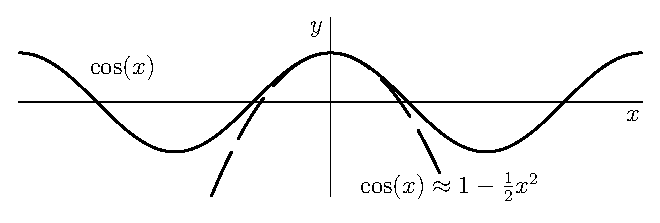
\includegraphics[width=300pt]{ChapterPowerSeries/Figures/cosdeg2.eps}
	\end{center}

\item {\bf Solving for $a_3$:} Yet again we differentiate and then plug in zero to find the coefficient $a_3$.
\begin{align*}
\left(-\cos(x)\right)'&=\left(2a_2+3\cdot 2a_3x+4\cdot 3 a_4x^2+5\cdot 4  a_5 x^3+\cdots\right)' \\
\sin(x)&=3\cdot 2a_3+4\cdot 3\cdot 2 a_4x+5\cdot 4 \cdot  3 a_5 x^2+\cdots \\
\sin(0)&=3\cdot 2a_3+4\cdot 3\cdot 2 a_4\cdot 0+5\cdot 4 \cdot  3 a_5\cdot  0^2+\cdots  \\
0&=3\cdot 2a_3 \\
a_3&=0 
\end{align*}
Graphically this makes sense; it is essentially saying that we couldn't represent cosine more accurately with a cubic polynomial function than we could have with a quadratic.  Near zero, the graph of cosine looks a lot more like a parabola than it does like the graph of a cubic.
 $$P_3(x)=1+0x-\frac{1}{2}x^2+0x^3 =1-\frac{1}{2}x^2$$

\item {\bf Solving for $a_4$:}  Yet again we differentiate and then plug in zero to find the coefficient $a_4$.
\begin{align*}
\left(\sin(x)\right)'&=\left(3\cdot 2a_3+4\cdot 3 \cdot 2 a_4x+5\cdot 4 \cdot 3 a_5 x^2+\cdots \right)' \\
\cos(x)&=4\cdot 3\cdot 2 a_4+5\cdot 4 \cdot 3 \cdot 2 a_5 x+ \cdots \\
\cos(0)&=4\cdot 3\cdot 2 a_4+5\cdot 4 \cdot 3 \cdot 2 a_5 \cdot 0+ \cdots \\
1&=4\cdot 3\cdot 2a_4 \\
a_4&=\frac{1}{4!} 
\end{align*}

 $$P_4(x)=1+0x-\frac{1}{2}x^2+0x^3+\frac{1}{4!}x^4 =1-\frac{1}{2}x^2+\frac{1}{24}x^4$$

	\begin{center}
		\includegraphics[width=300pt]{ChapterPowerSeries/Figures/cosdeg4.eps}
	\end{center}
\item {\bf Solving for $a_5$ and $a_6$:}  By a similar argument, we find $a_5=0$ and $a_6=-\frac{1}{6!}$.  Thus, we have the best sixth-degree polynomial approximation.

 $$P_6(x)=1-\frac{1}{2}x^2+\frac{1}{24}x^4-\frac{1}{6!}x^6$$
 
	\begin{center}
		\includegraphics[width=300pt]{ChapterPowerSeries/Figures/cosdeg6.eps}
	\end{center}

\end{itemize}

From here we see the pattern: 
\begin{itemize}
\item {\bf Left-hand Side:} The derivatives will continue cycling through the four functions $\cos(x), -\sin(x), -\cos(x), $ and $\sin(x)$.  When we plug in $x=0$, these functions give us the numbers $1, 0, -1,$ and 0 respectively.

\item {\bf Right-hand Side:} After $n$ derivatives, the only term that will not have a power of $x$ attached to it is of the form $n!a_n$.  We then must divide both sides by $n!$ to solve for $a_n$. 
\end{itemize}

Extrapolating this pattern, we can state the full power series for cosine. $$\cos(x)=1-\frac{1}{2!}x^2+\frac{1}{4!}x^4-\frac{1}{6!}x^6+\frac{1}{8!}x^8-\cdots $$

Often, we condense our notation by writing the power series in sigma notation rather than in expanded form as follows:

$$ \cos(x)=\sum_{n=0}^\infty (-1)^{n}\frac{1}{\left(2n\right)!}x^{2n}.$$
\end{example}

\newpage

Ok, you know what has to happen next. 

\begin{exercise}{Time for Sine \Coffeecup \Coffeecup}
Repeat the above process to find the \sine{power series} for sine!

\vspace*{7in}
\AnswerKeyEntry{Written in sigma notation, the power series is $\sin(x)=\Sigma_{n=0}^\infty (-1)^{n}\frac{1}{\left(2n+1\right)!}x^{2n+1}$.}
\end{exercise}

\newpage
And again.

\begin{exercise}{The Exponential Function \Coffeecup \Coffeecup}
Repeat the above process to find the power series for the natural exponential function, $f(x)=e^x$.
\vspace*{7in}
\AnswerKeyEntry{Written in sigma notation, the power series is $e^x=\Sigma_{n=0}^\infty \frac{1}{n!}x^{n}$.}
\end{exercise}

\newpage

And again.

\begin{exercise}{A Familiar Function \Coffeecup \Coffeecup}
\begin{itemize} \item Repeat the above process to find the power series for the function $f(x)=\frac{1}{1-x}$.

\vspace*{5.5in}
\item How does the above \geometricseries{power series} relate to the geometric series formula?
\vspace*{1in}
\end{itemize}
\AnswerKeyEntry{The power series is $\frac{1}{1-x}=\Sigma_{n=0}^\infty x^n$.  It is a geometric series with initial term 1 and common ratio $x$.}
\end{exercise}

This method can be considered the \powerseries{brute force method} of finding a power series.  Later, we will develop more efficient methods, but this is how we get off the ground!  Let us sum up (heh) this method below.

\begin{center}
\tcbox[left=0mm,right=0mm,top=0mm,bottom=0mm,boxsep=0mm,toptitle=0.5mm,bottomtitle=0.5mm,center title,title=Brute Force Method for Finding a Power Series]{\renewcommand*{\arraystretch}{1.8}%
\begin{tabular}{l}
       To find a power series for a function $f(x)$, carry out the following steps:  \\

\textbullet Write down the form of an unknown power series. \\
       $f(x)=a_0+a_1x+a_2x^2+a_3x^3+a_4x^4+a_5x^5+\cdots $ \\
\textbullet Plug in $x=0$ to solve for $a_0$. \\
\textbullet Differentiate both sides and plug in $x=0$ to solve for $a_1$. \\
\textbullet Differentiate both sides and plug in $x=0$ to solve for $a_2$. \\
\textbullet Repeat this until you have as many terms as you need! \vspace*{0.5cm} \\
	\multicolumn{1}{c}{
		\vspace*{0.5cm}
		\begin{tikzpicture}[
      >=latex',
      auto
    ]
    
    \tikzstyle{box} = [rectangle, rounded corners, minimum width=2cm, minimum height=1cm, text centered, text width=2.7cm, draw=black, fill=gray!15, drop shadow]
    
    \tikzstyle{arrow} = [thick,>=stealth,arrowhead=5mm,->]
    
    \node [box] (xZero) {
    	Plug in $x=0$
        };
     \node [box]  (solve) [node distance=0.7cm and -.5cm,below right=of xZero] {
     	Solve for next coefficient
     	};
	\node [box]  (diff) [node distance=0.7cm and -0.5cm,below left=of xZero] {
     	Differentiate
     	};
    
    \draw [->, >=open triangle 60, ultra thick,line width= 3pt, shorten >=2pt] (xZero.east) -- ($(xZero.east)+(0.25,0)$) -| (solve.north);
    \draw [->, >=open triangle 60, ultra thick,line width= 3pt, shorten >=2pt] (solve.west) --  (diff.east);
    \draw [->, >=open triangle 60, ultra thick,line width= 3pt, shorten >=2pt] (diff.north) -- ($(diff.north)+(0,0.7)$) |- (xZero.west);

\end{tikzpicture}
	}
    \end{tabular} }
\end{center}

Often this method is called \emph{Taylor's Formula}.  The key idea is to notice that to solve for the coefficient $a_n$, we must differentiate exactly $n$ times and then divide by $n!$.  We rewrite this below in a more formulaic manner. 

\begin{theorem}{\taylorseries{Taylor's Formula}}
If $f(x)$ and all of its derivatives are defined at $x=0$, then 
\begin{align*}
f(x)&=f(0)+f'(0)x+\frac{f''(0)}{2!}x^2+\frac{f'''(0)}{3!}x^3+\cdots \\
  &=\sum_{n=0}^\infty \frac{f^{(n)}(0)}{n!}x^n
\end{align*}
for any value of $x$ for which the sum converges.
\end{theorem}

While the method above works for many functions, it sometimes fails.  In particular, it was no coincidence that the natural logarithm was absent from our examples above!

\begin{exercise}{Natural Log \Coffeecup \Coffeecup}
Try to find a \logarithms{power series} by our brute force method on the function $f(x)=\ln(x)$.  Where does it fail?
\vspace*{2in}
\AnswerKeyEntry{When we try to plug in $x=0$ to find $a_0$, we get $\ln(0)$ which is not a real number.}
\end{exercise}

To work around this, we adopt a more flexible view of power series.  Rather than attempting to write our function as a sum of powers of $x$, which requires the function and its derivatives to be defined at $x=0$, we express it as a sum of powers of $\left(x-a\right)$ for some real number $a$.  It is essentially the same process, but to solve for the coefficients, you would set $x=a$ instead of $x=0$.  This produces a power series \powerseries{centered at $a$}.  We state this method below: 


\begin{center}
\tcbox[left=0mm,right=0mm,top=0mm,bottom=0mm,boxsep=0mm,toptitle=0.5mm,bottomtitle=0.5mm,center title,title=Finding a Power Series Centered at $a$]{\renewcommand*{\arraystretch}{1.8}%
\begin{tabular}{l}
       To find a power series centered at $a$ for a function $f(x)$, carry out the following steps: \\

\textbullet Write down the form of an unknown power series centered at $a$. \\
       $f(x)=a_0+a_1(x-a)+a_2(x-a)^2+a_3(x-a)^3+a_4(x-a)^4+\cdots $ \\
\textbullet Plug in $x=a$ to solve for $a_0$. \\
\textbullet Differentiate both sides and plug in $x=a$ to solve for $a_1$. \\
\textbullet Differentiate both sides and plug in $x=a$ to solve for $a_2$. \\
\textbullet Repeat this until you have as many terms as you need! \vspace*{0.5cm} \\
	\multicolumn{1}{c}{
		\vspace*{0.5cm}
		\input{ChapterPowerSeries/Figures/bruteforcea}
	}
    \end{tabular} }
\end{center}

\begin{exercise}{Natural Log, Again \Coffeecup \Coffeecup}
Use the upgraded brute force method to find a \logarithms{power series} for $f(x)=\ln(x)$ centered at $1$. \vspace*{6in}
\AnswerKeyEntry{The power series centered at one for the natural log is $\ln(x)=\Sigma_{n=1}^\infty\frac
{(-1)^{n+1}}{n}(x-1)^n$.}
\end{exercise}

\subsection{Binomial Series}\label{BuyNoMealSeries}

The next exercise constructs the \binomialseries{binomial series}, an extremely important series in the fields of combinatorics, probability, and statistics.

\begin{exercise}{Binomial Series \Coffeecup \Coffeecup \Coffeecup}
Let $m\in\mathbb{R}$.  A function of the form $$f(x)=\left(1+x\right)^m $$ is called a \emph{binomial}, since it has two terms in the polynomial inside parentheses.  Let us run the brute force method on this function to find its power series, the \emph{binomial series}.     

\begin{itemize}
\item Use the brute force method to find the first five terms in the series.  \vspace*{3in}

\item Since that is cumbersome to write down, we define the \emph{binomial coefficient} ``$m$ choose $n$'' to be the following: 

$$\binom{m}{n}=\frac{m\cdot (m-1) \cdot (m-2) \cdots (m-n+1)}{n!} $$ For example, $\binom{7}{3}=\frac{7\cdot 6\cdot 5}{3!}=35$.

Demonstrate that with this notation, the terms you found via brute force are equivalent to the series $$\left( 1+x\right)^m=\sum_{n=0}^\infty\binom{m}{n}x^n. $$ 

\vspace*{2in}

\end{itemize}

\end{exercise}

\newpage

\begin{exercise}{Understanding Binomial Coefficient Notation \Coffeecup}

In the formula for the binomial coefficient $\binom{m}{n}$, how many numbers are multiplied together in the numerator? \vspace*{1in}

\end{exercise}

Note that $m$ was not restricted to being a whole number.  Since it could be fractional, the binomial series allows us to rewrite radicals as polynomials!  

\begin{example}{Power Series of a Cubed Root}
Suppose we wish to find a degree three power series for the function $$f(x)=\sqrt[3]{1+x}. $$

We apply the Binomial Series with $m=1/3$. Proceeding, we have

\begin{align*}
f(x)&=\sqrt[3]{1+x}\\
&=\sum_{n=0}^\infty\binom{1/3}{n}x^n\\
&=\binom{1/3}{0}+\binom{1/3}{1}x+\binom{1/3}{2}x^2+\binom{1/3}{3}x^3+\cdots \\
&=\frac{1}{0!}+\frac{\left(1/3\right)}{1!}x+\frac{\left(1/3\right)\left(-2/3\right)}{2!}x^2+\frac{\left(1/3\right)\left(-2/3\right)\left(-5/3\right)}{3!}x^3+\cdots \\
&=1+\frac{1}{3}x-\frac{1}{9}x^2+\frac{5}{81}x^3+\cdots. \\
\end{align*}

Thus, the best degree three polynomial approximation of $f(x)$ centered at zero is $$ \sqrt[3]{1+x}\approx 1+\frac{1}{3}x-\frac{1}{9}x^2+\frac{5}{81}x^3.$$
\end{example}